\section{One-Step Generative Modeling}
\label{sec:onestep}

Building on the flow matching framework, recent methods have developed increasingly sophisticated techniques for learning one-step or few-step generators. We discuss four representative velocity-based approaches: consistency flow matching, which enforces straightness through velocity consistency; shortcut models, which learn via self-consistency bootstrapping; mean flows, which train from scratch using the mean-flow identity; and AlphaFlow, which unifies these ideas through curriculum learning. All four methods share a common lineage through consistency models, as discussed in \cref{subsec:consistency-models}.

\subsection{Consistency Flow Matching}
\label{subsec:consistencyfm}

Consistency Flow Matching (Consistency-FM) \citep{zhou2024consistency} proposes to enforce \emph{velocity consistency} along flow trajectories. Unlike rectified flow, which iteratively straightens trajectories through repeated simulation and retraining, Consistency-FM directly defines straight flows by imposing a self-consistency constraint on the velocity field itself. This avoids both the computational cost of optimal transport approximations and the accumulation error of multi-stage rectification.

\begin{figure}[htbp]
  \centering
  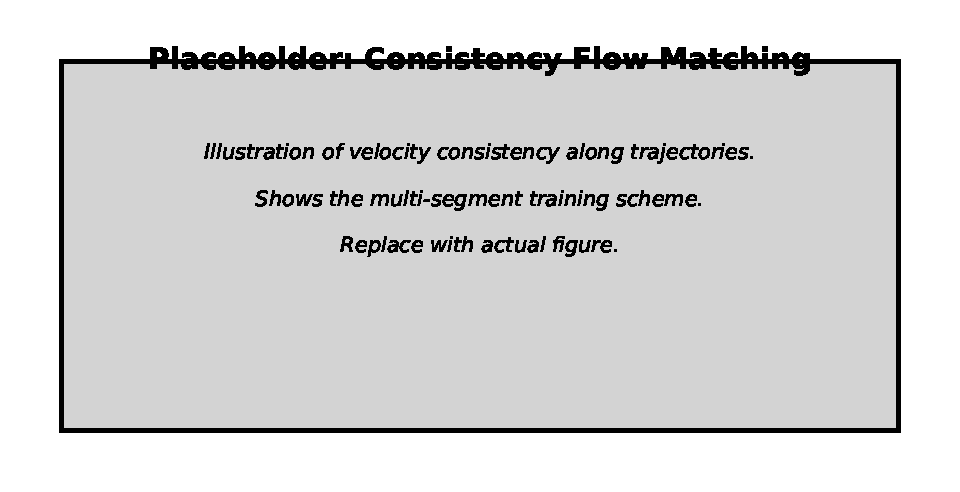
\includegraphics[width=0.8\linewidth]{Figures/figure_consistency_fm.pdf}
  \caption{Placeholder: Illustration of Consistency Flow Matching velocity consistency. Replace with a figure showing the multi-segment training scheme.}
  \label{fig:placeholder-consistency-fm}
\end{figure}

\paragraph{Velocity consistency.} Given a flow trajectory $z_t$ with learned velocity $v_\theta(t, z_t)$, the core idea is to require the velocity to be constant along each trajectory:
\begin{equation}
    v(t, z_t) = v(r, z_r) \quad \forall t, r \in [0,1].
    \label{eq:cfm-cond1}
\end{equation}
However, imposing \cref{eq:cfm-cond1} alone admits trivial solutions (e.g., $v_\theta \equiv 0$). The key theoretical insight is an equivalence lemma \citep{zhou2024consistency}: under mild regularity conditions, \cref{eq:cfm-cond1} is equivalent to a trajectory-level condition
\begin{equation}
    z_t + (1-t) \, v(t, z_t) = z_r + (1-r) \, v(r, z_r),
    \label{eq:cfm-cond2}
\end{equation}
which requires the quantity $f_\theta(t, z_t) \triangleq z_t + (1-t) \, v_\theta(t, z_t)$ to be invariant along the path. At $t = 1$ (the noise endpoint), this quantity evaluates to $\epsilon$, and by invariance it predicts the data sample at any $t$, thereby tying the consistency constraint to the data distribution itself.

\paragraph{Training objective.} The loss enforces both \cref{eq:cfm-cond1,eq:cfm-cond2} between nearby timesteps:
\begin{equation}
    \mathcal{L}_\theta = \mathbb{E}_{t, z_t, z_{t+\Delta t}} \Big[ \| f_\theta(t, z_t) - f_{\theta^-}(t+\Delta t, z_{t+\Delta t}) \|^2 + \lambda \| v_\theta(t, z_t) - v_{\theta^-}(t+\Delta t, z_{t+\Delta t}) \|^2 \Big],
\end{equation}
where $\theta^-$ is an EMA of the parameters and $\lambda$ balances the two terms. The first term enforces endpoint consistency (trajectory invariance of $f_\theta$), while the second regularizes the velocity field. An asymptotic analysis \citep{zhou2024consistency} shows that minimizing this loss interpolates between two desiderata: matching the ground-truth velocity field (as in standard FM), and enforcing a consistency condition on the velocity's material derivative $\partial_t v_\theta + u \cdot \nabla v_\theta$, which drives the velocity toward constancy along trajectories. \Cref{alg:consistency_fm} summarizes one training iteration.

\paragraph{Multi-segment training.} For complex distributions where a single straight trajectory is insufficient, Consistency-FM divides $[0,1]$ into $K$ equal segments and learns a separate consistent velocity $v_\theta^i$ within each segment $[i/K, (i+1)/K]$. Each segment obeys its own version of the loss with the endpoint adjusted to the segment boundary, yielding piecewise-linear trajectories that can approximate curved transport paths. The theoretical analysis further shows that if the ground-truth velocity is consistent within a segment, Consistency-FM recovers it exactly (up to the oracle velocity), providing a formal error bound on the learned field.

\paragraph{One-step sampling.} Under perfect velocity consistency, the velocity field is constant along each trajectory: $v(t, z_t) = v(0, x) = \epsilon - x$. Since the ODE $dz_t/dt = v$ is linear with constant velocity, integrating backward from $t=1$ to $t=0$ yields $x = \epsilon - v_\theta(\epsilon, 1)$. In practice, a single network evaluation at $t=1$ produces a one-step generation.

\begin{algorithm}[t]
\caption{Consistency Flow Matching Training}
\label{alg:consistency_fm}
\begin{algorithmic}[1]
\Require Data $x_1$, noise $x_0$, velocity network $v_\theta$, EMA model $v_{\theta^-}$, optimizer, hyperparameter $\alpha$
\State Sample $t \sim \text{Uniform}(0, 1 - \Delta t)$
\State $x_t \gets (1 - t) \, x_0 + t \, x_1$
\State $x_{t+\Delta t} \gets (1 - (t+\Delta t)) \, x_0 + (t+\Delta t) \, x_1$
\State $v_t \gets v_\theta(x_t, t)$
\State $v_{t+\Delta t} \gets v_\theta(x_{t+\Delta t}, t+\Delta t)$
\State $f_t \gets x_t + (1 - t) \, v_t$
\State $f_{t+\Delta t} \gets x_{t+\Delta t} + (1 - (t+\Delta t)) \, v_{t+\Delta t}$
\State \Comment{with no grad}
\State $f_{t+\Delta t}^{\text{ema}} \gets x_{t+\Delta t} + (1 - (t+\Delta t)) \, v_{\theta^-}(x_{t+\Delta t}, t+\Delta t)$
\State $f_t^{\text{ema}} \gets x_t + (1 - t) \, v_{\theta^-}(x_t, t)$
\State $\mathcal{L}_f \gets \| f_t - f_{t+\Delta t}^{\text{ema}} \|^2 + \| f_{t+\Delta t} - f_t^{\text{ema}} \|^2$
\State $\mathcal{L}_v \gets \| v_t - v_{\theta^-}(x_{t+\Delta t}, t+\Delta t) \|^2 + \| v_{t+\Delta t} - v_{\theta^-}(x_t, t) \|^2$
\State $\mathcal{L} \gets \mathcal{L}_f + \alpha \, \mathcal{L}_v$
\State Update $\theta$ with $\nabla_\theta \mathcal{L}$; update EMA model
\State \Return $\mathcal{L}$
\end{algorithmic}
\end{algorithm}


\subsection{Shortcut Models}
\label{subsec:shortcut}

Shortcut Models \citep{frans2024shortcut} approach one-step generation through a self-consistency principle. The key insight is that a single large step along the probability-flow ODE must be consistent with two consecutive smaller steps that span the same interval. Unlike Consistency-FM, which enforces consistency in the instantaneous velocity field, shortcut models directly learn a mapping conditioned on the desired step size.

\begin{figure}[htbp]
  \centering
  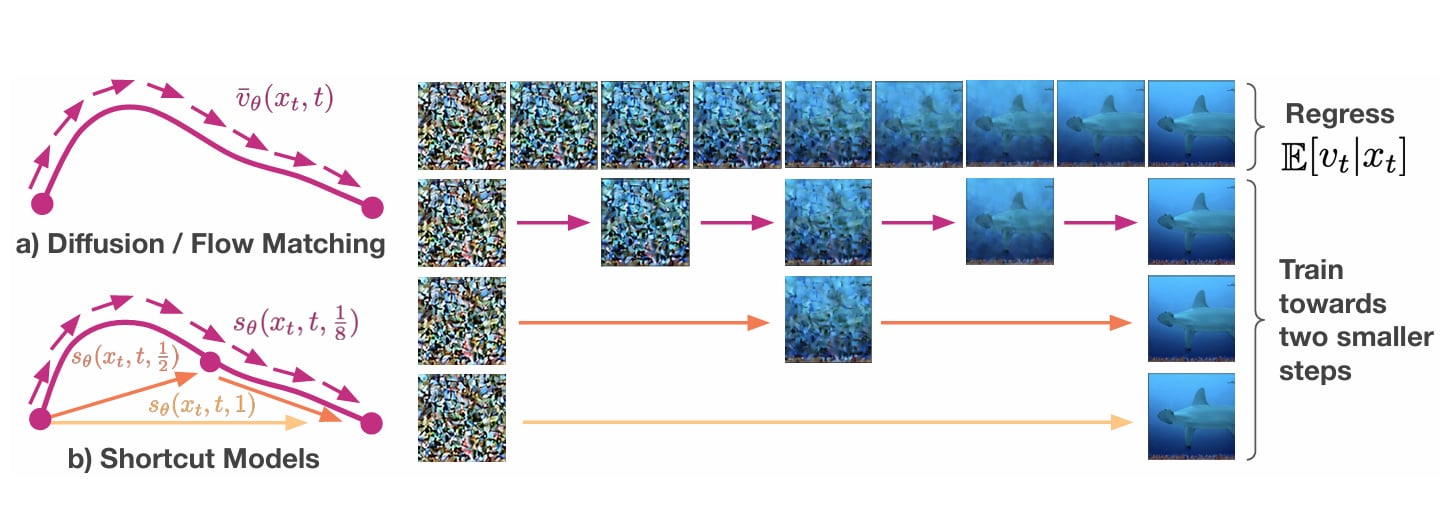
\includegraphics[width=\linewidth]{Figures/Shortcut.png}
  \caption{Training schematic for shortcut models \citep{frans2024shortcut}. When the interval length $d \equiv t - r$ approaches zero, the model reverts to standard flow matching by directly predicting the conditional velocity $\epsilon - x$. For larger $d$, the target is bootstrapped by chaining two half-interval shortcuts and averaging their outputs, enforcing self-consistency across step sizes. Both regimes are optimized jointly in a single training phase.}
  \label{fig:shortcut}
\end{figure}

The model learns a \emph{shortcut} $s_\theta(z_t, r, t)$ that predicts the average velocity from the current (later) time $t$ to a target (earlier) time $r$ ($r < t$). Given the state $z_t$ and the interval $[r, t]$, a single step toward data is:
\begin{equation}
    z_r = z_t - (t - r) \, s_\theta(z_t, r, t).
\end{equation}
For one-step generation, starting from noise $z_1 = \epsilon$ and setting $r=0, t=1$ yields $x = \epsilon - s_\theta(\epsilon, 0, 1)$.

The training objective exploits a \emph{self-consistency} decomposition: a shortcut over a large interval can be expressed as the average of two consecutive shortcuts over half-intervals. Let $m = (r + t)/2$ be the midpoint:
\begin{equation}
    s(z_t, r, t) = \frac{s(z_t, m, t) + s(z_m, r, m)}{2},
    \label{eq:sc-self-consistency}
\end{equation}
where $z_m = z_t - (t - m) \, s_\theta(z_t, m, t)$ is obtained by following the first half-step prediction. This yields the self-consistency training loss:
\begin{equation}
    \mathcal{L}_{\text{SC}}(\theta) = \mathbb{E}_{r,t,x,\epsilon} \Big[ \big\| s_\theta(z_r, r, t) - \text{sg}\Big( \frac{1}{2} \big( s_\theta(z_r, r, m) + s_\theta(z_m, m, t) \big) \Big) \big\|^2 \Big],
    \label{eq:sc-loss}
\end{equation}
where $\text{sg}$ denotes the stop-gradient operator.

To ground the model at small step sizes, shortcut models include a flow matching base case. As $t \to r$, the shortcut reduces to the instantaneous velocity, and the model is trained with standard flow matching:
\begin{equation}
    \mathcal{L}_{\text{FM}}(\theta) = \mathbb{E}_{t, \epsilon, x} \big\| s_\theta(z_t, t, t) - (\epsilon - x) \big\|^2.
\end{equation}
In practice, the training batch mixes a fraction $k$ of self-consistency samples ($r < t$) with $1 - k$ flow matching samples ($r = t$), yielding a combined objective trained jointly in a single phase. \Cref{alg:shortcut_models} details the training procedure.

\begin{algorithm}[t]
\caption{Shortcut Model Training}
\label{alg:shortcut_models}
\begin{algorithmic}[1]
\Require Data $x$, noise $\epsilon$, shortcut network $s_\theta$, optimizer, self-consistency ratio $k$
\State Sample $r, t \sim \text{Uniform}(0,1)$ with $r < t$
\State $z_t \gets (1 - t) \, x + t \, \epsilon$ \Comment{Interpolant at later time}
\State $v \gets \epsilon - x$ \Comment{Conditional velocity}
\If{flow-matching base case ($r = t$)}
    \State $s_{\text{tgt}} \gets v$ \Comment{Flow matching target}
\Else
    \State $m \gets (r + t) \,/\, 2$ \Comment{Midpoint}
    \State $s_1 \gets s_\theta(z_t, m, t)$
    \State $z_m \gets z_t - (t - m) \cdot s_1$ \Comment{First half-step (toward data)}
    \State $s_2 \gets s_\theta(z_m, r, m)$
    \State $s_{\text{tgt}} \gets \text{sg}\big( (s_1 + s_2) / 2 \big)$ \Comment{Self-consistency target}
\EndIf
\State $\mathcal{L} \gets \| s_\theta(z_t, r, t) - s_{\text{tgt}} \|^2$
\State Update $\theta$ with $\nabla_\theta \mathcal{L}$
\State \Return $\mathcal{L}$
\end{algorithmic}
\end{algorithm}


A key practical advantage of shortcut models is that they require no JVP computation: the self-consistency target is constructed from two additional forward passes rather than through derivatives. This makes training computationally cheaper than JVP-based methods, with only $\sim 16\%$ more compute than a standard flow-matching model. Furthermore, shortcut models can be trained end-to-end from scratch without a pre-trained teacher, distillation stages, or carefully scheduled curricula. \Cref{fig:shortcut} illustrates this training procedure: at $d \approx 0$ the objective reduces to standard flow matching, while targets for larger step sizes are bootstrapped by composing two half-sized shortcuts.

\subsection{Mean Flows}
\label{subsec:meanflow}

Mean Flow \citep{geng2025mean} addresses a fundamental limitation of previous methods: the reliance on pre-trained teacher models or expensive distillation pipelines. It proposes a principled framework for one-step generative modeling that can be trained from scratch.

\begin{figure}[htbp]
  \centering
  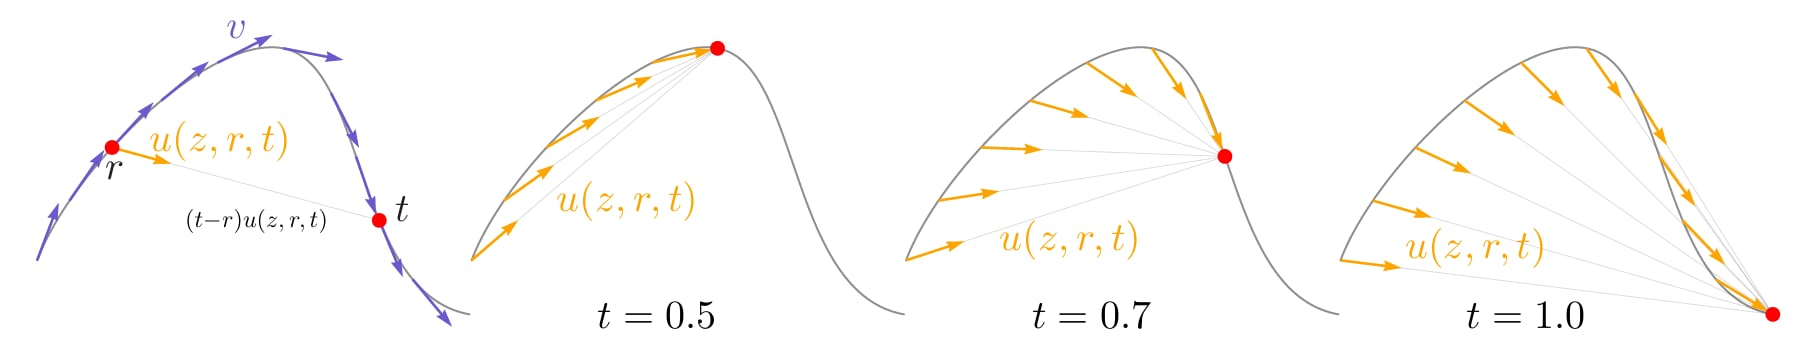
\includegraphics[width=\linewidth]{Figures/MeanFlow.jpg}
  \caption{Visualization of the average velocity field $u(z, r, t)$ \citep{geng2025mean}. \textbf{Left:} Unlike the instantaneous velocity $v$, which gives the local tangent direction, the average velocity $u$ points along the chord connecting $z_t$ to $z_r$ and generally differs in direction from $v$. \textbf{Right three panels:} The average velocity depends on both the earlier time $r$ and the later time $t$, shown for $t = 0.5$, $0.7$, and $1.0$ respectively.}
  \label{fig:mean-flows-field}
\end{figure}

The key insight is to model the \emph{average velocity} rather than the instantaneous velocity. For a trajectory $z_t$, the average velocity between times $r$ and $t$ is defined as:
\begin{equation}
    u(z_t, r, t) = \frac{1}{t-r} \int_r^t v(z_\tau, \tau) \, d\tau.
\end{equation}
While the instantaneous velocity $v$ determines the tangent direction of the path, the average velocity $u$ is aligned with the net displacement $(t-r)\,u$ and is generally not parallel to $v$; \cref{fig:mean-flows-field} visualizes this field for several values of $t$. Differentiating the definition $(t-r)u = \int_r^t v \, d\tau$ with respect to $t$ yields the \emph{MeanFlow Identity}:
\begin{equation}
    u(z_t, r, t) = v(z_t, t) - (t-r) \frac{d}{dt} u(z_t, r, t),
\end{equation}
where the total derivative $\frac{d}{dt} u = v \cdot \partial_z u + \partial_t u$ is computed efficiently as a Jacobian-Vector Product (JVP).

The training objective, outlined in \cref{alg:mean_flows}, regresses the network prediction $u_\theta$ against the target derived from the MeanFlow Identity:
\begin{equation}
    \mathcal{L}(\theta) = \mathbb{E} \| u_\theta(z_t, r, t) - \text{sg}\big(v(z_t, t) - (t-r)(v(z_t, t) \cdot \partial_z u_\theta + \partial_t u_\theta)\big) \|^2,
\end{equation}
where $\text{sg}$ denotes the stop-gradient operator.

\begin{algorithm}[t]
\caption{MeanFlow Training}
\label{alg:mean_flows}
\begin{algorithmic}[1]
\Require Data $x$, noise $\epsilon$, average-velocity network $u_\theta$, optimizer
\State Sample $r, t \sim \text{Uniform}(0,1)$ with $r < t$
\State $z_t \gets (1 - t) \, x + t \, \epsilon$ \Comment{Interpolant}
\State $v \gets \epsilon - x$ \Comment{Instantaneous conditional velocity}
\State $u_{\text{pred}} \gets u_\theta(z_t, r, t)$
\State Compute JVP: $(v, 1) \cdot \nabla u_\theta(z_t, r, t)$ \Comment{Total derivative $\frac{d}{dt} u$}
\State $u_{\text{tgt}} \gets v - (t - r) \cdot \frac{d}{dt} u$ \Comment{MeanFlow Identity}
\State $\mathcal{L} \gets \| u_{\text{pred}} - \text{sg}(u_{\text{tgt}}) \|^2$
\State Update $\theta$ with $\nabla_\theta \mathcal{L}$
\State \Return $\mathcal{L}$
\end{algorithmic}
\end{algorithm}


\paragraph{Classifier-free guidance.} MeanFlow bakes classifier-free guidance (CFG) directly into the training objective, avoiding the standard approach of combining conditional and unconditional outputs at inference time (which would double NFE). The key idea is to define a CFG-augmented ground-truth velocity field:
\begin{equation}
    v^{\text{cfg}}(z_t, t \mid \mathbf{c}) \triangleq \omega \, v(z_t, t \mid \mathbf{c}) + (1-\omega) \, v(z_t, t),
\end{equation}
with an associated CFG average velocity $u^{\text{cfg}}$ that satisfies the same MeanFlow Identity. Crucially, the unconditional component $v(z_t, t)$ is replaced in the training target by the network's own unconditional prediction $u_\theta^{\text{cfg}}(z_t, t, t)$, yielding a self-contained objective:
\begin{equation}
    \tilde{v}_t \triangleq \omega \, v_t + (1-\omega) \, u_\theta^{\text{cfg}}(z_t, t, t),
\end{equation}
which serves as the $\tilde{v}_t$ that feeds into the MeanFlow Identity in place of $v(z_t, t)$. Because the average velocity $u_\theta^{\text{cfg}}$ directly models the CFG-augmented field, \textbf{no additional combination is needed at sampling time}: a single evaluation $x = \epsilon - u_\theta^{\text{cfg}}(\epsilon, 0, 1 \mid \mathbf{c})$ produces a guided one-step sample. AlphaFlow adopts the same CFG formulation, detailed in \cref{subsec:alphaflow}.

\paragraph{One-step sampling.} Given a trained MeanFlow model, one-step generation follows directly from the definition of the average velocity. Since $z_r = z_t - (t-r) \, u_\theta(z_t, r, t)$, setting $r=0$ and $t=1$ yields:
\begin{equation}
    x = \epsilon - u_\theta(\epsilon, 0, 1).
\end{equation}
This requires a single forward pass of the network, with no iterative ODE integration. With CFG enabled, the same formula applies using $u_\theta^{\text{cfg}}$ in place of $u_\theta$, preserving the 1-NFE property.



\subsection{AlphaFlow}
\label{subsec:alphaflow}

AlphaFlow \citep{zhang2025alphaflow}\footnote{Official implementation: \url{https://github.com/snap-research/alphaflow}.} addresses a subtle but important limitation of MeanFlow: the MeanFlow objective is actually composed of two competing terms whose gradients conflict during training. By decomposing the objective and resolving this conflict through curriculum learning, AlphaFlow improves both convergence and final sample quality.

\begin{figure}[htbp]
  \centering
  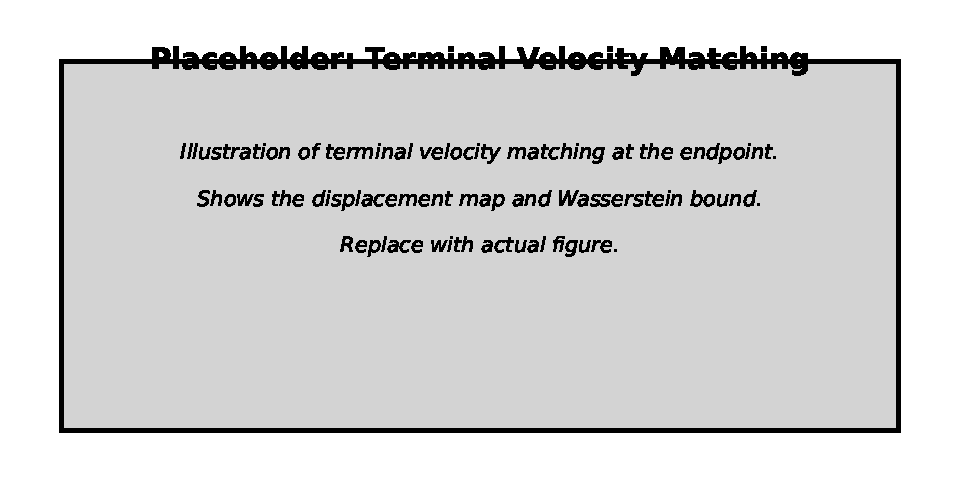
\includegraphics[width=0.8\linewidth]{Figures/figure_terminal_velocity.pdf}
  \caption{Placeholder: Illustration of the AlphaFlow curriculum. Replace with a figure showing the interpolation between trajectory flow matching ($\alpha=1$) and MeanFlow ($\alpha \to 0$).}
  \label{fig:placeholder-alphaflow}
\end{figure}


The starting point is the observation that the MeanFlow loss can be rewritten as the sum of a \emph{trajectory flow matching} term and a \emph{trajectory consistency} term:
\begin{equation}
    \mathcal{L}_{\text{MF}}(\theta) = \underbrace{\mathbb{E}_{t,r,z_t} \big[ \| u_\theta(z_t, r, t) - v_t \|^2 \big]}_{\mathcal{L}_{\text{TFM}}} + \underbrace{\mathbb{E}_{t,r,z_t} \big[ 2(t-r) \, u_\theta(z_t, r, t)^\top \tfrac{d}{dt} u_{\theta^\text{-}}(z_t, r, t) \big]}_{\mathcal{L}_{\text{TC}_c}} + C,
\end{equation}
where $C$ is independent of $\theta$. Empirically, the gradients of $\mathcal{L}_{\text{TFM}}$ and $\mathcal{L}_{\text{TC}_c}$ are strongly negatively correlated, which makes joint optimization unstable and slows convergence. The large flow-matching ratio used in MeanFlow ($r=t$ for 75\% of samples) can be understood as a surrogate that reduces this conflict, but it also consumes most of the training budget on a border case.

To unify and disentangle these objectives, AlphaFlow introduces a single interpolation parameter $\alpha \in (0, 1]$:
\begin{equation}
    \mathcal{L}_\alpha(\theta) = \mathbb{E}_{t,r,z_t} \Big[ \alpha^{-1} \big\| u_\theta(z_t, r, t) - \big( \alpha v_t + (1-\alpha) u_{\theta^\text{-}}(z_s, r, s) \big) \big\|^2 \Big],
\end{equation}
where $s = \alpha r + (1-\alpha)t$ and $z_s = z_t + (t-s) v_t$. This family recovers several previous methods as special cases: $\alpha = 1$ gives trajectory flow matching; $\alpha = 1/2$ corresponds to the Shortcut Model objective; and $\alpha \to 0$ recovers MeanFlow. With an endpoint parameterization ($r \equiv 0$), it also subsumes discrete and continuous consistency training.

The practical training schedule proceeds in three phases. First, the model is pretrained with $\alpha = 1$ (trajectory flow matching) to quickly reach a reliable noise-to-data mapping. Then $\alpha$ is annealed smoothly toward 0, transitioning from the low-variance flow-matching objective to the low-bias MeanFlow objective. Finally, the model is fine-tuned with $\alpha \approx 0$. \Cref{alg:alphaflow} illustrates this curriculum. Because the early phase already optimizes trajectory flow matching, AlphaFlow requires far less border-case flow-matching supervision than MeanFlow while achieving better final performance.

\begin{algorithm}[t]
\caption{AlphaFlow Training}
\label{alg:alphaflow}
\begin{algorithmic}[1]
\Require Data $x$, noise $\epsilon$, average-velocity network $u_\theta$, iteration $k$, schedule $\alpha(k)$, optimizer
\State Sample $r, t \sim \text{Uniform}(0,1)$ with $r < t$
\State $\alpha \gets \alpha(k)$; \quad $s \gets \alpha r + (1-\alpha) t$
\State $z_t \gets (1 - t) \, x + t \, \epsilon$ \Comment{Interpolant}
\State $v \gets \epsilon - x$ \Comment{Conditional velocity}
\If{$\alpha = 0$}
    \State $u \gets u_\theta(z_t, r, t)$
    \State Compute JVP: $\tfrac{d}{dt} u_\theta(z_t, r, t)$
    \State $u_{\text{tgt}} \gets v - (t - r) \cdot \tfrac{d}{dt} u$ \Comment{MeanFlow target}
\Else
    \State $u \gets u_\theta(z_t, r, t)$
    \State $z_s \gets z_t + (t - s) \cdot v$
    \State $u_{\text{tgt}} \gets \alpha v + (1 - \alpha) \, u_{\theta^\text{-}}(z_s, r, s)$ \Comment{Interpolated target}
\EndIf
\State $\mathcal{L} \gets \alpha^{-1} \| u - \text{sg}(u_{\text{tgt}}) \|^2$
\State Update $\theta$ with $\nabla_\theta \mathcal{L}$
\State \Return $\mathcal{L}$
\end{algorithmic}
\end{algorithm}


\paragraph{One-step sampling.} Since AlphaFlow shares the same average-velocity parameterization $u_\theta$, its one-step sampling is identical to MeanFlow: $x = \epsilon - u_\theta(\epsilon, 0, 1)$. For few-step generation, AlphaFlow can employ either ODE sampling or consistency sampling, selecting the intermediate timestep that yields the best trade-off between FID and FDD. AlphaFlow adopts the same CFG formulation as MeanFlow (\cref{subsec:meanflow}), baking guidance into the training target so that a single NFE suffices for guided generation.

